\documentclass[11pt]{amsart}

\usepackage{a4wide}
\usepackage[usenames,dvipsnames]{color}
\usepackage[latin1]{inputenc}
\usepackage[catalan]{babel}
\usepackage{paralist}
\usepackage{graphicx}
\usepackage{times}

\newcommand{\obert}{\textcolor{red}{\bfseries Obert\ }}
\newcommand{\falta}{\textcolor{red}{\bfseries Falta\ }}
\newcommand{\progres}{\textcolor{BurntOrange}{\bfseries En progr�s\ }}
\newcommand{\complert}{\textcolor{ForestGreen}{\bfseries Complert\ }}


\begin{document}

\title{l'Admin Blau: Requisits}
\maketitle


\section{Descripci� de les entitats principals de l'aplicaci�}

\begin{description}
\item[Castellers] \complert
\item[Categories de castellers] \complert
\item[Rols] \complert; sense funcionalitat
\item[Fam�lies] \progres definit, crud funciona; \falta taula intermitjana per persones
\item[Quotes]\progres crud parcial; \falta poder editar b� els responsables i coberts 
\item[Esdeveniments] \progres \falta preus
\item[Compte] \falta
\item[Rebuts] \falta
\end{description}


\section{Requisits funcionals}

\subsection{Versi� 1.0}
\begin{description}
\item[R01] Alta, baixa i modificaci� de persones \complert
\item[R02] Agrupar persones per fam�lies \progres
\item[R03] Alta, baixa i modificaci� de quotes \progres
\item[R04] Generaci� de rebuts \falta
\end{description}

\subsection{Versi� 2.0}

\newpage
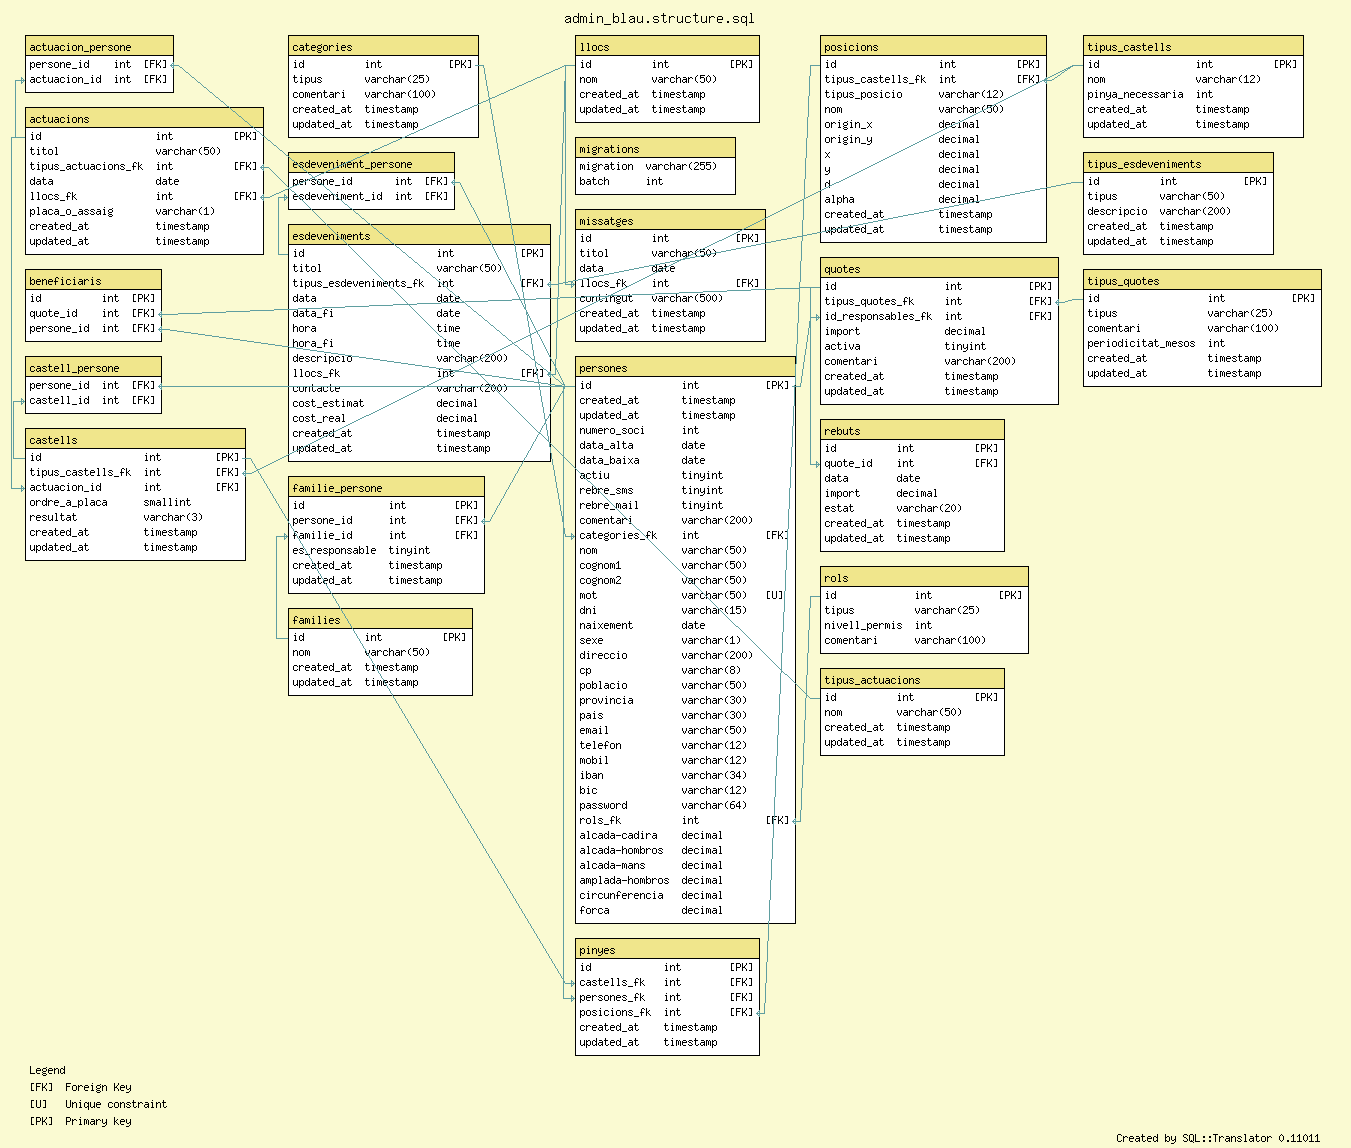
\includegraphics[width=\linewidth]{DbSchemaAdminBlau}

\end{document}
